\section{Methods of Measuring Aerosol}

Two fundamental methods are used to measure aerosols concentrations within the atmosphere. The first of these methods are ground based and in-situ measurements which give good detail and information about a specific localized. However, these measurements are limited in scope has they do not have global coverage that is inherent in satellite instrumentation. Both ground base and satellites have important roles in monitoring the planets aerosol content, however each of these methods have inherent advantages and disadvantages. A overview will be given of some of the common methods to determine aerosol concentration and why using different methods helps to increase the overall accuracy and precision of data sets.

\subsection{In-Situ}

In-situ measurement have occurs on balloon based platform in which particle counters are used. Balloon instruments that use particle counters during the assent direct count the aerosol particle as well can determine the particle size distributions. One such instruments is the Optical Particle Counter (OPC) is an active light source instrument that has a incandescent light source internal to the device. The instrument has been launched from Laramie, Wyoming since 1971. The instrument measures the internal light source using the forward scatter at a central angle of 25\si{\degree} over a approximately 30\si{\degree} solid angle to determine aerosol extinction and particle size \citep{Rosen1964, Deshler2003}. A second type of in-situ balloon instruments uses a passive light source, including the sun, moon, or stars, to determine aerosol extinctions. Instruments that use this type of technology are the Absorption par les Minoritaires Ozone et $\text{NO}_{\text{x}}$ (AMON) from 1992 to 2003 and Spectroscopie d\si{\arcminute}Absorption Lunaire pour l\si{\arcminute}Observation des Minoritaires Ozone et $\text{NO}_{\text{x}}$ - Nacelle 2 (SALOMON-N2) from 2007 onwards which use starlight and moon light respectively \citep{Berthet2002}. In-situ measurements of aerosol extinction give direct measurement of scattered light from the altitude that the balloon is currently situated, which helps to reduce scattered light contamination from aerosol particles at different altitudes especially for instruments that use an active light source. This allows for a most possible isolated aerosol measurements  and direct measurement of aerosol extinction and cross section unlike remote sensing applications from satellites. However, these types of instrument due not active global coverage of aerosol measurements and only give aerosol extinction from a very localized region, like OPC, or have very few flights, for example AMON which had a total of six stratospheric balloon flights, three mid-latitude northern and three high-latitude northern flights. In order to achieve full global coverage satellite remote sensing instruments were create to fill the spatial gap.

\subsection{LIDAR}

Through the transmission of a laser pulse though the atmosphere, a method known as LIght Dectection and Ranging (LIDAR) can determine aerosol concentrations through the measuring of the intensity of the backscattered laser light at different wavelengths and polarizations.

\begin{figure}[h]
    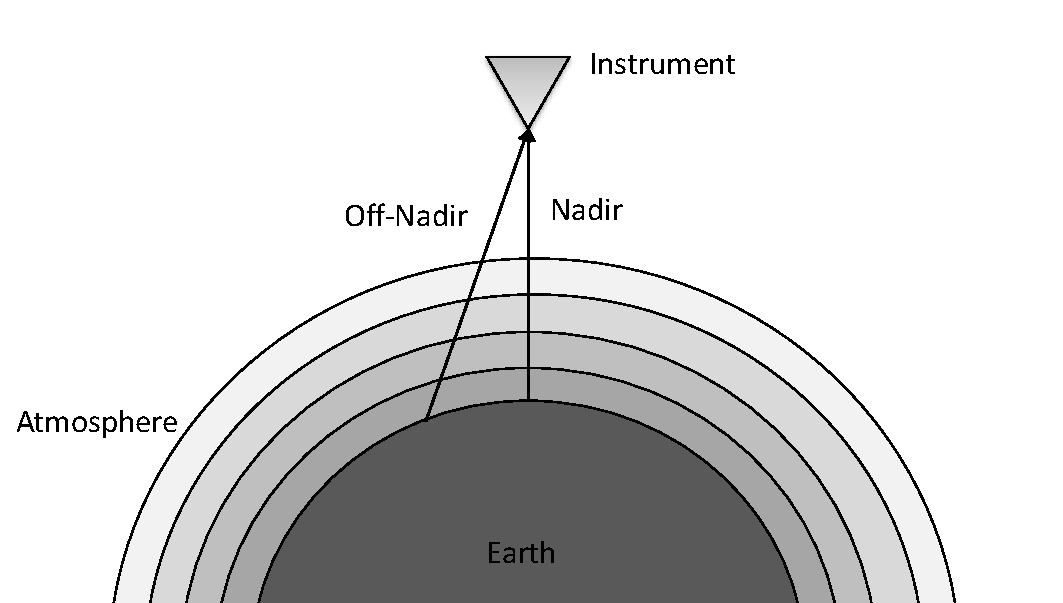
\includegraphics[width=1.0\textwidth]{./Images/LidarGeometry.pdf}
    \caption[LIDAR Geometry]{LIDAR instrument showing a measurement in both the nadir and offnadir lines of sight.}
    \label{fig:LidarGeometry}
\end{figure}

\subsection{Occultation}

SAGE II SAGE III SAM II

\subsection{Limb Emission}

MIPAS and MLS (I think) now have sulphate products

\subsection{Limb Scatter}
\subsubsection{Scanning}

SCIAMACHY OSIRIS

\subsubsection{Imaging}

OMPS and ALTIUS 